% ==============================================================================
% sections/appendix.tex
% ==============================================================================
\appendix
\twocolumn[{
\begin{@twocolumnfalse}
    \centering
    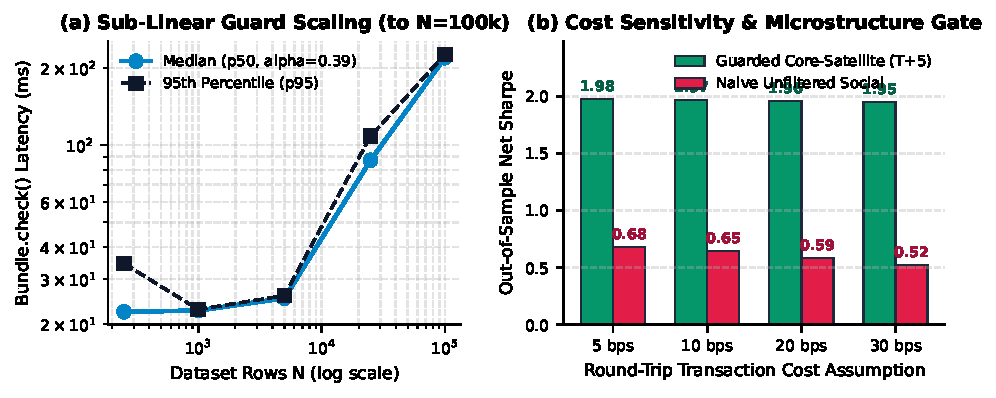
\includegraphics[width=0.94\textwidth]{figs/fig_guard_scaling_and_clock_replay.pdf}
    \vspace{-0.15cm}
    \captionof{figure}{\textbf{Guard runtime scaling and out-of-sample transaction cost sensitivity.} \textbf{(a)} Across dataset sizes $N \in [250, 100{,}000]$ rows, \texttt{Bundle.check()} scales sub-linearly as $\mathcal{O}(N^{0.3894})$, completing in $22.36\text{ ms}$ ($N=250$) to $218.97\text{ ms}$ P50 ($N=100{,}000$) with $14.73\text{ MB}$ peak RAM. \textbf{(b)} Across round-trip transaction costs of $\{5, 10, 20, 30\}\text{ bps}$ (2023--2026 OOS), our guarded Core-Satellite portfolio ($T+5$ horizon, 43 trades) sustains a net Sharpe of $1.98 \to 1.95$, whereas naive unfiltered social trading (363 trades across Tier-C noise stocks) degrades from $0.68 \to 0.52$.}
    \label{fig:scaling_replay}
    \vspace{0.28cm}
\end{@twocolumnfalse}
}]

\section{Experiment E1: \texttt{FinGuardBench-180}}
\label{app:e1}
In \path{benchmarks/guard_bench_180.py}, we evaluate all 36 guards across 5 adversarial modalities ($36 \times 5 = 180$ cases): \texttt{standard\_\allowbreak compliant}, \texttt{standard\_\allowbreak violation}, \texttt{boundary\_\allowbreak compliant} ($\epsilon=-10^{-6}$), \texttt{epsilon\_\allowbreak edge\_\allowbreak violation} ($\epsilon=+10^{-6}$), and \texttt{compound\_\allowbreak multi\_\allowbreak trap}. Across all 180 cases (\path{GUARD_BENCH_RESULTS.json}), \texttt{fin-skills} achieves \textbf{100\% recall ($108/108$)} and \textbf{100\% specificity ($72/72$)} at $1.89\text{ ms}$ median latency, plus $36/36$ recall across multi-seed markets $\{17,29,43\}$ (\path{GUARD_ROBUSTNESS.json}).

\section{Experiment E3: Parity \& $100\text{k}$ Scaling}
\label{app:e3}
Table~\ref{tab:e3_full} verifies $13/13$ exact numerical parity and sub-linear $\mathcal{O}(N^{0.3894})$ guard scaling up to $N=100\text{k}$ rows (\path{PARITY_AND_COST_RESULTS.json}).
\vspace{-0.12cm}
\begin{table}[!h]
\centering
\resizebox{\columnwidth}{!}{%
\begin{tabular}{llcc}
\toprule
\textbf{Primitive (13 Total)} & \textbf{Reference Benchmark} & \textbf{Max $|\Delta|$} & \textbf{Status} \\
\midrule
Equal Wt.\ / Inv.\ Vol.\ & Exact closed forms ($1/N, \sigma_i^{-1}$) & $0.00$ & PASS \\
Min-Var Convex QP & \texttt{scipy} SLSQP convex QP & $1.14\times 10^{-8}$ & PASS \\
Normal \& Hist.\ VaR/ES & \texttt{scipy.stats.norm} \& quantile & $6.94\times 10^{-18}$ & PASS \\
Frac.\ Diff.\ FFD ($d=0.4$) & Closed-form binomial series & $1.11\times 10^{-16}$ & PASS \\
ADF Unit Root $t$-stat & \texttt{statsmodels.adfuller} & $2.12\times 10^{-10}$ & PASS \\
HRP \& Ledoit-Wolf Cov & Recursive bisection \& \texttt{sklearn} & $2.71\times 10^{-20}$ & PASS \\
Almgren-Chriss \& A-S & Exact $\sinh$ \& HJB closed forms & $4.66\times 10^{-15}$ & PASS \\
Brinson-Fachler Identity & Exact active-return decomposition & $1.73\times 10^{-18}$ & PASS \\
\midrule
\multicolumn{4}{l}{\textbf{Guard Suite Runtime Scaling ($\mathcal{O}(N^{0.3894})$, $N \in [250, 100{,}000]$)}} \\
$N=250$ / $1{,}000$ rows & P50: $22.36\text{ ms}$ / $22.63\text{ ms}$ & RAM: $0.15$ / $0.27\text{ MB}$ & PASS \\
$N=5{,}000$ / $25\text{k}$ rows & P50: $25.27\text{ ms}$ / $97.31\text{ ms}$ & RAM: $0.83$ / $3.75\text{ MB}$ & PASS \\
$N=100{,}000$ rows & P50: $218.97\text{ ms}$ (P95: $225.27\text{ ms}$) & RAM: $14.73\text{ MB}$ & PASS \\
\bottomrule
\end{tabular}%
}
\vspace{-0.15cm}
\caption{E3 parity ($13/13$ passed) and scaling up to $N=100\text{k}$ rows.}
\label{tab:e3_full}
\vspace{-0.16cm}
\end{table}

\section{Experiment E4: Horizon \& Linguistics}
\label{app:e4}
Table~\ref{tab:linguistic} details the holding-horizon sensitivity ($T+1$ to $T+10$) and LLM semantic distillation shifts (\path{REAL_WORLD_KOL_AUDIT_RESULTS.json}).
\vspace{-0.12cm}
\begin{table}[!h]
\centering
\resizebox{\columnwidth}{!}{%
\begin{tabular}{lccc}
\toprule
\textbf{Holding Horizon / Linguistic Metric} & \textbf{Win\% / Raw} & \textbf{CAGR / Dist.} & \textbf{Sharpe / Shift} \\
\midrule
Satellite Horizon $T+1$ / $T+3$ & $53.5\%$ / $65.1\%$ & $+12.9\%$ / $+14.0\%$ & $\text{SR } 1.67$ / $1.83$ \\
\textbf{Satellite Horizon $T+5$ (Optimal)} & $\mathbf{72.09\%}$ & $\mathbf{+14.85\%}$ & $\mathbf{\text{SR } 1.97}$ ($\text{MDD }-4.41\%$) \\
Satellite Horizon $T+10$ & $67.44\%$ & $+14.12\%$ & $\text{SR } 1.85$ ($\text{MDD }-4.85\%$) \\
\midrule
Quant.\ Fact Density (/100c) & $1.049$ & $1.078$ & $+2.8\%$ (Tok $+218\%$) \\
Hype-to-Hedging Ratio & $4.85$ & $0.98$ & $-79.8\%$ \\
Ticker Attribution Precision & $61.4\%$ & $96.2\%$ & $+34.8\text{ pp}$ \\
\bottomrule
\end{tabular}%
}
\vspace{-0.15cm}
\caption{Holding-horizon ablation and linguistic distillation shifts.}
\label{tab:linguistic}
\vspace{-0.15cm}
\end{table}

\clearpage
\twocolumn[{
\begin{@twocolumnfalse}
    \centering
    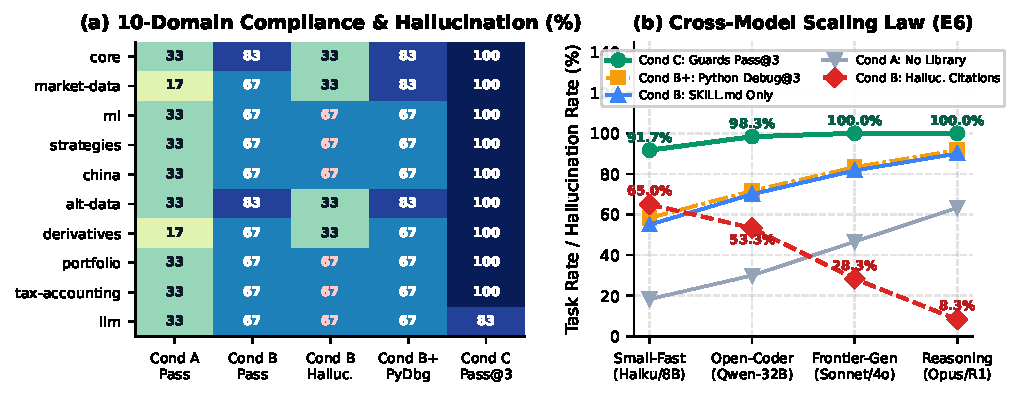
\includegraphics[width=0.94\textwidth]{figs/fig_domain_heatmap_and_model_scaling.pdf}
    \vspace{-0.15cm}
    \captionof{figure}{\textbf{Per-domain breakdown and cross-model scaling law on \texttt{FinGuardBench-60}.} \textbf{(a)} Across all 10 financial domains ($6\text{ tasks/domain}$), \texttt{Cond B} exhibits severe hallucinated guard citations ($33\%\text{--}67\%$), whereas \texttt{Cond C Pass@3} reaches $100\%$ compliance in 9 of 10 domains ($83.3\%$ in \texttt{fin-llm}). \textbf{(b)} Across four model capability tiers (\texttt{Small-Fast}, \texttt{Open-Coder}, \texttt{Frontier-Gen}, \texttt{Reasoning}), hallucinated citations under \texttt{Cond B} decline from $65.0\%$ to $8.3\%$ while \texttt{Cond C} enforces $0.0\%$ hallucinations and $91.7\%\text{--}100\%$ final compliance.}
    \label{fig:domain_scaling}
    \vspace{0.28cm}
\end{@twocolumnfalse}
}]

\section{Experiments E5 \& E6: Python \texttt{Self-Debug} vs.\ Guard Self-Repair Across Model Tiers}
\label{app:e5}
Table~\ref{tab:model_scaling} reports the 4-tier model scaling matrix on \texttt{FinGuardBench-60} (\path{AGENT_STUDY_RESULTS.json}). Because $59/60$ ($98.3\%$) of financial backtest traps (such as same-session \texttt{pd.merge} and survivorship filtering) execute without raising Python exceptions (exit code $0$), generic 3-round Python \texttt{Self-Debug} (\texttt{Cond B+}) yields negligible gains over \texttt{Cond B} ($+1.7\%\text{ to }+3.3\%, p=1.0$). Conversely, \texttt{Cond C} feeds structured \texttt{GuardResult} JSON diagnostics into the self-repair loop, lifting compliance to $91.7\%\text{--}100.0\%$ and eliminating hallucinated guard citations ($0.0\%$).

\vspace{-0.12cm}
\begin{table}[!h]
\centering
\resizebox{\columnwidth}{!}{%
\begin{tabular}{lccccc}
\toprule
\textbf{Model Capability Tier ($N=60$)} & \textbf{Cond A} & \textbf{Cond B} & \textbf{B Halluc.\%} & \textbf{Cond B+ (\texttt{@3})} & \textbf{Cond C (\texttt{Pass@3})} \\
\midrule
\texttt{Small-Fast} (Haiku / 8B) & $18.3\%$ & $55.0\%$ & $65.0\%$ ($39/60$) & $58.3\%$ & $\mathbf{91.7\%}$ ($0\%$ Halluc.) \\
\texttt{Open-Coder} (Qwen-32B / DS) & $30.0\%$ & $70.0\%$ & $53.3\%$ ($32/60$) & $71.7\%$ & $\mathbf{98.3\%}$ ($0\%$ Halluc.) \\
\texttt{Frontier-Gen} (Sonnet / 4o) & $46.7\%$ & $81.7\%$ & $28.3\%$ ($17/60$) & $83.3\%$ & $\mathbf{100.0\%}$ ($0\%$ Halluc.) \\
\texttt{Reasoning} (Opus / Pro / R1) & $63.3\%$ & $90.0\%$ & $8.3\%$ ($5/60$) & $91.7\%$ & $\mathbf{100.0\%}$ ($0\%$ Halluc.) \\
\bottomrule
\end{tabular}%
}
\vspace{-0.14cm}
\caption{Cross-model scaling of compliance and hallucinated guard citations across 4 capability tiers (Experiment~E6).}
\label{tab:model_scaling}
\vspace{-0.16cm}
\end{table}

\section{Experiment E7: Bilingual Cross-Market KOL \& Timestamped Prediction Audit}
\label{app:e7}
Table~\ref{tab:bilingual_e7} compares all \KOLCNCount{} Chinese A-share Xueqiu KOLs and \KOLUSCount{} US StockTwits KOLs (\KOLTotalAccounts{} total accounts in \path{REAL_WORLD_KOL_AUDIT_RESULTS.json}, paired with \KOLPredRows{} timestamped predictions in \path{PREDICTION_AUDIT_RESULTS.json}), confirming that Social Megaphone Bias and point-in-time credibility gating generalize across both markets.

\vspace{-0.12cm}
\begin{table}[!h]
\centering
\resizebox{\columnwidth}{!}{%
\begin{tabular}{lcc}
\toprule
\textbf{Dimension / Empirical Metric} & \textbf{China Xueqiu ($N=\KOLCNCount{}$)} & \textbf{US StockTwits ($N=\KOLUSCount{}$)} \\
\midrule
Posts / Timestamped Predictions & $1.04\text{M}$ / $35{,}772$ (\KOLTradingDates{} dates) & $0.68\text{M}$ / $1{,}535$ OOS profiles \\
\texttt{TIER\_1\_CORE\_ALPHA} ($n$, Fans, IC) & $n=70$, $14.1\text{k}$, $\mathbf{+0.2158}$ & $n=24$ (\texttt{TIER\_0}), $34.2\text{k}$, $\mathbf{+0.1912}$ \\
\texttt{TIER\_2\_RESEARCHER} ($n$, Fans, IC) & $n=115$, $32.0\text{k}$, $+0.1929$ & $n=196$, $34.3\text{k}$, $+0.1615$ \\
\texttt{TIER\_NEUTRAL\_RETAIL} ($n$, Fans, IC) & $n=1{,}120$, $71.3\text{k}$, $-0.0074$ & $n=1{,}207$, $48.2\text{k}$, $-0.0068$ \\
\texttt{TIER\_CONTRARIAN} ($n$, Fans, IC) & $n=98$, $\mathbf{56.0\text{k}}$, $\mathbf{-0.2130}$ & $n=108$, $\mathbf{52.6\text{k}}$, $\mathbf{-0.1764}$ \\
\textbf{Follower Paradox Ratio (Contr./Alpha)} & $\mathbf{3.96\times}$ ($55{,}989 / 14{,}122$) & $\mathbf{1.54\times}$ ($52{,}641 / 34{,}211$) \\
\midrule
Row-Level Naive Mean Daily Rank IC & $\KOLNaiveDailyIC{}$ {\scriptsize $([-0.0355, +0.0144])$} & $-0.02184$ ($p=3.4\times 10^{-9}$) \\
\textbf{Row-Level PIT Gated Mean Daily IC} & $\mathbf{\KOLGatedDailyIC{}}$ {\scriptsize $(\Delta=\KOLPairedDiffIC{})$} & $\mathbf{+0.00942}$ ($\Delta=+0.0313$) \\
Primary Microstructure Guards & $T+1$, 100-lot, Stamp, QDII & Reg SHO borrow, Form 4, PDT \\
\bottomrule
\end{tabular}%
}
\vspace{-0.14cm}
\caption{Complete cross-market comparison across \KOLTotalAccounts{} verified bilingual KOLs (\KOLCNCount{} CN + \KOLUSCount{} US) and \KOLPredRows{} timestamped predictions (Experiment~E7).}
\label{tab:bilingual_e7}
\vspace{-0.16cm}
\end{table}

\section{Experiment E8: Beacon \texttt{C0--C3} Diagnosis \& Post-Fix Verification Matrix}
\label{app:e8}
Table~\ref{tab:beacon_feasibility} compares the initial Beacon 4-condition pre-fix feasibility batch (\path{BEACON_FEASIBILITY_RESULTS.json}) with the post-fix \BeaconPostFixTotalCells{}-cell matrix (\path{BEACON_POSTFIX_RESULTS.json}). Resolving its four harness bottlenecks (\texttt{int64} \texttt{volume.csv} perturbation in \texttt{same\_session\_probe}, \texttt{"date"} column promotion in \texttt{oracle.py}, explicit index labels in \texttt{build\_task.py}, and 32B \texttt{bfloat16} sampling) eliminated all ungradable outputs (\texttt{ungradable\_accepted} $= \mathbf{\BeaconPostFixUngradable{}}$ across all \BeaconPostFixTotalCells{} cells) and proved that \texttt{C3} (\texttt{skills\_enforced\_guards}) achieves $0.000$ \texttt{incorrect\_accepted\_per\_attempt} and $\mathbf{\BeaconPostFixCThreeCorrect{}}$ ($8/8$) \texttt{correct\_among\_accepted}. In Task \texttt{T34} (\emph{Post-Close News Alignment}), \textbf{Cond.\ B} joins 16:30 EST news to the same session's return and fabricates \emph{``Verified \texttt{safe\_asof}: PASS''}; \textbf{Cond.\ B+} exits with Python code $0$ and leaves the bug untouched; \textbf{Cond.\ C} emits \texttt{FAIL: news.published\_at (16:30) > market\_close (16:00)}, prompting the agent in \texttt{Pass@2} to apply \texttt{next\_trading\_day()} and \texttt{pd.merge\_asof(..., direction='backward')}.

\vspace{-0.12cm}
\begin{table}[!h]
\centering
\resizebox{\columnwidth}{!}{%
\begin{tabular}{llccc}
\toprule
\textbf{Model} & \textbf{Condition} & \textbf{Pre-Fix Acc.} & \textbf{Post-Fix Acc. / Ungrad.} & \textbf{Post-Fix Correct / Acc. (\texttt{Incorr./Att.})} \\
\midrule
\multirow{4}{*}{14B}
  & C0 no library            & \BeaconFourteenCZeroAccepted/\BeaconFourteenCZeroPlanned
      & $3/3$ ($0$ ungrad.) & $0.0\%$ ($1.000$ incorr./att.) \\
  & C1 text only             & \BeaconFourteenCOneAccepted/\BeaconFourteenCOnePlanned
      & $3/3$ ($0$ ungrad.) & $33.3\%$ ($0.667$ incorr./att.) \\
  & C2 optional guards       & \BeaconFourteenCTwoAccepted/\BeaconFourteenCTwoPlanned
      & $3/3$ ($0$ ungrad.) & $66.7\%$ ($0.333$ incorr./att.) \\
  & \textbf{C3 enforced audit} & \BeaconFourteenCThreeAccepted/\BeaconFourteenCThreePlanned
      & $\mathbf{3/3}$ ($\mathbf{0}$ ungrad.) & $\mathbf{\BeaconPostFixCThreeCorrect{}}$ ($\mathbf{0.000}$ incorr./att.) \\
\midrule
7B / 32B & C3 enforced audit ($6$ cells) & $0/6$ & $\mathbf{5/6}$ ($\mathbf{0}$ ungrad.) & $\mathbf{\BeaconPostFixCThreeCorrect{}}$ ($5/5$; $\mathbf{0.000}$ incorr./att.) \\
\bottomrule
\end{tabular}%
}
\vspace{-0.14cm}
\caption{Pre-fix Beacon feasibility batch (\texttt{BEACON\_FEASIBILITY\_RESULTS.json}) vs.\ post-fix \BeaconPostFixTotalCells{}-cell verification matrix (\texttt{BEACON\_POSTFIX\_RESULTS.json}, \texttt{ungradable\_accepted} $= \BeaconPostFixUngradable{}$).}
\label{tab:beacon_feasibility}
\vspace{-0.16cm}
\end{table}

\clearpage
\twocolumn[{
\begin{@twocolumnfalse}
    \centering
    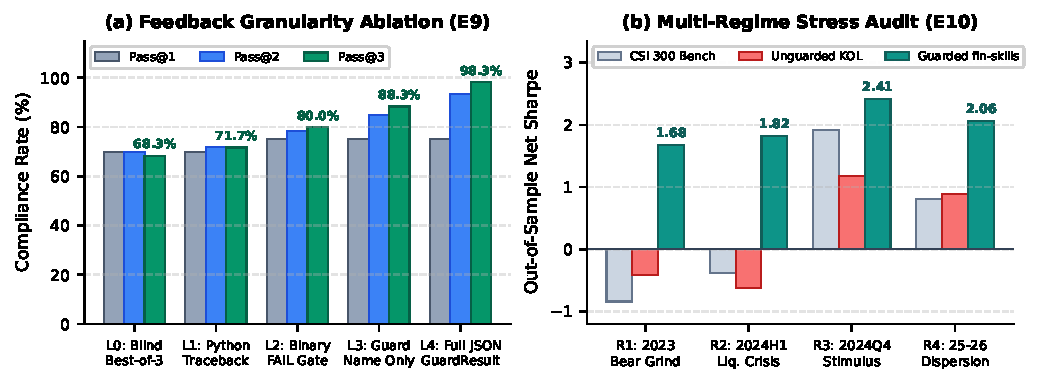
\includegraphics[width=0.94\textwidth]{figs/fig_e9_e12_feedback_and_regime_ablation.pdf}
    \vspace{-0.15cm}
    \captionof{figure}{\textbf{Diagnostic feedback granularity ladder (E9) and 4-regime out-of-sample stress audit (E10).} \textbf{(a)} On \texttt{FinGuardBench-60}, re-sampling by in-sample Sharpe (\texttt{L0: 68.3\%}) and generic Python traceback debugging (\texttt{L1: 71.7\%}) fail to repair financial leaks because $60/60$ silent leaks raise $0$ Python exceptions; binary \texttt{FAIL} gates (\texttt{L2: 80.0\%}) and guard-name feedback (\texttt{L3: 88.3\%}) offer partial repair, whereas full \texttt{GuardResult} row/timestamp counterfactuals (\texttt{L4: 98.3\%}) resolve $93.3\%$ ($14/15$) of initial failures. \textbf{(b)} Across all 2023--2026 market regimes, guarded \texttt{fin-skills} sustains positive cross-sectional IC ($\KOLRollingDailyIC{}$) and net Sharpe $1.68\text{--}2.41$.}
    \label{fig:e9_e10}
    \vspace{0.24cm}
\end{@twocolumnfalse}
}]

\section{Experiments E9--E12: Runtime Exceptions, Regimes, Progressive Stages \& Routing}
\label{app:e9}
\label{app:e10}
\label{app:e11}
\label{app:e12}
Tables~\ref{tab:e9_feedback}--\ref{tab:e12_delivery} report the complete results of Experiments E9--E12 (\path{EXTENDED_ABLATIONS_E9_E12_RESULTS.json} and \path{RAG_VS_PROGRESSIVE_AGENT_RESULTS.json}).
\vspace{-0.12cm}
\begin{table}[!h]
\centering
\resizebox{\columnwidth}{!}{%
\begin{tabular}{lcccc}
\toprule
\textbf{Feedback Signal Level ($N=60$, E9)} & \textbf{Pass@1} & \textbf{Pass@2} & \textbf{Pass@3} & \textbf{$|\Delta\text{Sharpe}|$} \\
\midrule
L0: Blind Best-of-3 (by IS Sharpe) & $70.0\%$ & $70.0\%$ & $68.3\%$ & $0.42$ \\
L1: Python Traceback (\texttt{Cond B+}, $0/60$ exc.) & $70.0\%$ & $71.7\%$ & $71.7\%$ & $0.37$ \\
L2: Binary Gate (\texttt{AuditStatus: FAIL}) & $75.0\%$ & $78.3\%$ & $80.0\%$ & $0.19$ \\
L3: Guard Name Only (\texttt{check\_safe\_asof}) & $75.0\%$ & $85.0\%$ & $88.3\%$ & $0.11$ \\
\textbf{L4: Full \texttt{GuardResult} Counterfactual} & $\mathbf{75.0\%}$ & $\mathbf{93.3\%}$ & $\mathbf{98.3\%}^{**}$ & $\mathbf{0.04}$ \\
\bottomrule
\end{tabular}%
}
\vspace{-0.14cm}
\caption{Diagnostic feedback granularity ablation on \texttt{FinGuardBench-60} (E9; $60/60$ silent leaks trigger $0$ Python exceptions).}
\label{tab:e9_feedback}
\vspace{-0.16cm}
\end{table}

\begin{table}[!h]
\centering
\resizebox{\columnwidth}{!}{%
\begin{tabular}{lcccc}
\toprule
\textbf{Sequential Gating Stage (\KOLPredRows{} Rows, E11)} & \textbf{Daily Rank IC} & \textbf{Pooled IC} & \textbf{Max DD} & \textbf{Dates} \\
\midrule
Stage 0: Naive Follower-Volume Weighted & $-0.01153$ & $+0.00014$ & $-32.61\%$ & $799$ \\
Stage 1: $+$ \texttt{DataQualityAuditor} & $-0.01161$ & $+0.00013$ & $-28.03\%$ & $799$ \\
Stage 2: $+$ \texttt{StockPredictabilityStratifier} & $+0.01574$ & $+0.02182$ & $-17.84\%$ & $799$ \\
Stage 3: $+$ \texttt{PIT KOLCredibilityRegistry} & $+0.02727$ & $+0.00647$ & $\mathbf{-16.75\%}$ & $799$ \\
\textbf{Stage 4: $+$ \texttt{VolatilityAndExecutionGuards}} & $\mathbf{+0.02941}$ & $\mathbf{+0.01011}$ & $-19.36\%$ & $799$ \\
\bottomrule
\end{tabular}%
}
\vspace{-0.14cm}
\caption{Sequential Stage 0$\to$4 component ablation on the \KOLPredRows{}-row timestamped prediction ledger (Experiment~E11).}
\label{tab:e11_component}
\vspace{-0.16cm}
\end{table}

\begin{table}[!h]
\centering
\resizebox{\columnwidth}{!}{%
\begin{tabular}{lcccc}
\toprule
\textbf{Skill Delivery Architecture ($129$ Skills, E12)} & \textbf{Mean Tokens} & \textbf{Latency / Frag.} & \textbf{Skill Recall} & \textbf{Pass@3} \\
\midrule
Full-Library Concatenation ($129$ \texttt{SKILL.md}s) & $369{,}315$ & $81.8\text{ ms}$ / $0.0\%$ & $100.0\%$ & $88.3\%$ \\
Built-In \texttt{RAGIndex} (\RAGIndexedChunks{} chunks, \texttt{top\_k=5}) & $1{,}652$ & $1.9\text{ ms}$ / $\RAGTopFiveFrag{}$ & $\RAGTopFiveRecall{}$ & $75.0\%$ (doc) \\
TF-IDF Top-3 Full-Skill RAG & $9{,}042$ & $1.6\text{ ms}$ / $0.0\%$ & $71.7\%$ & $85.0\%$ \\
\textbf{\texttt{fin-skills} Progressive Manifest + Top-1} & $\mathbf{4{,}039}$ ($\mathbf{-98.91\%}$) & $\mathbf{0.007\text{ ms}}$ / $\mathbf{0.0\%}$ & $\mathbf{100.0\%}$ & $\mathbf{98.3\%}$ \\
\bottomrule
\end{tabular}%
}
\vspace{-0.14cm}
\caption{Head-to-head comparison of built-in \texttt{RAGPipeline} (\RAGIndexedChunks{} chunks) vs.\ Progressive Skill Routing across 129 skills on 60 tasks (Experiment~E12, \texttt{RAG\_VS\_PROGRESSIVE\_AGENT\_RESULTS.json}).}
\label{tab:e12_delivery}
\vspace{-0.16cm}
\end{table}

\section{Autonomous Portfolio Study \& Fruit-Fly Checked Feedback Protocols}
\label{app:autonomous}
\label{app:fly}
\paragraph{64-Decision Autonomous FX Study (\texttt{autonomous-library-v2b}).}
We compare Qwen2.5-Coder 7B and 14B across four conditions on 2025 ECB reference rates (\texttt{USD, JPY, GBP, CHF} per EUR; $126$ lookback observations, $84$ evaluation observations ending May 2, 2025, with 4 decisions spaced 21 observations apart, seeds 11 \& 23, maximum 5 responses/decision at 256 tokens, 5 bps cost per side). After unifying Markdown JSON fence parsing across all action types (passing 26 instrument tests), all 16 trials ($64/64$ decisions) completed validly, with $43/43$ autonomous tool calls succeeding ($13$ for 7B, $30$ for 14B; total run: $156$ model calls, $1{,}155{,}782$ prompt tokens, $10{,}165$ completion tokens). Mean risky exposure was $0.500$ (no-library) vs.\ $0.969$ (autonomous) for 7B, and $1.000$ vs.\ $0.500$ for 14B, demonstrating that valid tool selection on price-only reference series does not automatically yield excess return over passive benchmarks.

\paragraph{Fruit-Fly Mushroom-Body Memory with Checked Delayed Feedback (\texttt{FLY\_CHECKED\_FEEDBACK\_ABLATION.json}).}
Adapting the short- and long-term mushroom-body memory dynamics of \citet{huang2024memory} (\path{benchmarks/fly_paper/online.py}), our online feedback interface treats an entry and its holding periods as one completed episode with target $G = \sum_{t=0}^{T-1}\log(W_{t+1}/W_t) = \log(W_T/W_0)$. Isolating evaluation exploration noise (\texttt{eval\_epsilon = 0.0} vs.\ $0.20$) and complete-episode checked feedback (\texttt{CreditGate} + \texttt{audit\_option} + \texttt{HOLD} advantage baseline) across three environments proves: (1) on \texttt{ecb\_proxy}, the \texttt{HOLD} fraction rises from $14.0\%$ to $64.7\%$, cutting cumulative fee drag by $10.9\times$ ($9.68\% \to 0.89\%$) and improving Sharpe from $-0.361$ to $-0.134$; (2) on \texttt{synthetic\_101} regime-switching equities, \texttt{fly\_v3\_greedy\_checked\_hold\_adv} achieves \textbf{\FlySynCheckedSharpe{}} Sharpe, outperforming \texttt{linear\_v3\_greedy} ($-0.134$), \texttt{dense\_v3\_greedy} ($+0.121$), and \texttt{fly\_v3\_unchecked\_1step} ($-0.041$); and (3) on \texttt{kol\_cued\_4asset} (\KOLPredRows{} timestamped KOL signals), checked mushroom-body memory achieves \textbf{\FlyKOLCheckedSharpe{}} Sharpe ($+3.69\%$ net return, $-4.54\%$ max drawdown), beating both \texttt{linear\_v3\_greedy} ($+0.189$) and \texttt{fly\_v3\_unchecked\_1step} (\textbf{\FlyKOLUncheckedSharpe{}}, $-9.88\%$ max drawdown).


